\documentclass[border=10pt]{standalone}
\usepackage{tikz}
\begin{document}
\begin{tabular}{c}
$c^{(3, 2, 1)}_{(2, 1),\,(2, 1)} = 2$ \\[1em]
\textbf{Puzzle 1} \\[0.5em]
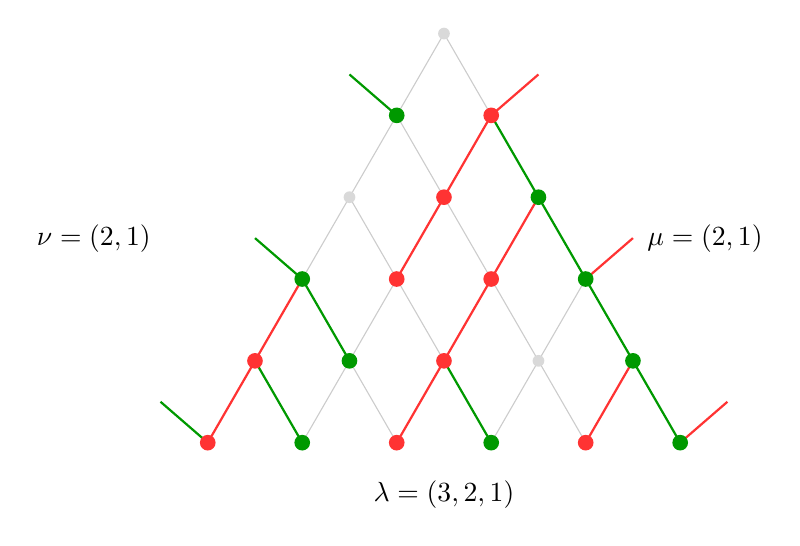
\begin{tikzpicture}[scale=1.2]
  \tikzstyle{reddot}=[circle, fill=red!80, inner sep=2pt]
  \tikzstyle{greendot}=[circle, fill=green!60!black, inner sep=2pt]
  \tikzstyle{emptydot}=[circle, fill=gray!30, inner sep=1.5pt]
  \tikzstyle{redline}=[red!80, thick]
  \tikzstyle{greenline}=[green!60!black, thick]
  \tikzstyle{grayline}=[gray!40, thin]
  \draw[redline] (0.000, 0.000) -- (0.500, 0.866);
  \draw[grayline] (1.000, 0.000) -- (1.500, 0.866);
  \draw[greenline] (1.000, 0.000) -- (0.500, 0.866);
  \draw[redline] (2.000, 0.000) -- (2.500, 0.866);
  \draw[grayline] (2.000, 0.000) -- (1.500, 0.866);
  \draw[grayline] (3.000, 0.000) -- (3.500, 0.866);
  \draw[greenline] (3.000, 0.000) -- (2.500, 0.866);
  \draw[redline] (4.000, 0.000) -- (4.500, 0.866);
  \draw[grayline] (4.000, 0.000) -- (3.500, 0.866);
  \draw[greenline] (5.000, 0.000) -- (4.500, 0.866);
  \draw[redline] (0.500, 0.866) -- (1.000, 1.732);
  \draw[grayline] (1.500, 0.866) -- (2.000, 1.732);
  \draw[greenline] (1.500, 0.866) -- (1.000, 1.732);
  \draw[redline] (2.500, 0.866) -- (3.000, 1.732);
  \draw[grayline] (2.500, 0.866) -- (2.000, 1.732);
  \draw[grayline] (3.500, 0.866) -- (4.000, 1.732);
  \draw[grayline] (3.500, 0.866) -- (3.000, 1.732);
  \draw[greenline] (4.500, 0.866) -- (4.000, 1.732);
  \draw[grayline] (1.000, 1.732) -- (1.500, 2.598);
  \draw[redline] (2.000, 1.732) -- (2.500, 2.598);
  \draw[grayline] (2.000, 1.732) -- (1.500, 2.598);
  \draw[redline] (3.000, 1.732) -- (3.500, 2.598);
  \draw[grayline] (3.000, 1.732) -- (2.500, 2.598);
  \draw[greenline] (4.000, 1.732) -- (3.500, 2.598);
  \draw[grayline] (1.500, 2.598) -- (2.000, 3.464);
  \draw[redline] (2.500, 2.598) -- (3.000, 3.464);
  \draw[grayline] (2.500, 2.598) -- (2.000, 3.464);
  \draw[greenline] (3.500, 2.598) -- (3.000, 3.464);
  \draw[grayline] (2.000, 3.464) -- (2.500, 4.330);
  \draw[grayline] (3.000, 3.464) -- (2.500, 4.330);
  \draw[greenline] (0.000, 0.000) -- (-0.500, 0.433);
  \draw[redline] (5.000, 0.000) -- (5.500, 0.433);
  \draw[greenline] (1.000, 1.732) -- (0.500, 2.165);
  \draw[redline] (4.000, 1.732) -- (4.500, 2.165);
  \draw[greenline] (2.000, 3.464) -- (1.500, 3.897);
  \draw[redline] (3.000, 3.464) -- (3.500, 3.897);
  \node[reddot] at (0.000, 0.000) {};
  \node[greendot] at (1.000, 0.000) {};
  \node[reddot] at (2.000, 0.000) {};
  \node[greendot] at (3.000, 0.000) {};
  \node[reddot] at (4.000, 0.000) {};
  \node[greendot] at (5.000, 0.000) {};
  \node[reddot] at (0.500, 0.866) {};
  \node[greendot] at (1.500, 0.866) {};
  \node[reddot] at (2.500, 0.866) {};
  \node[emptydot] at (3.500, 0.866) {};
  \node[greendot] at (4.500, 0.866) {};
  \node[greendot] at (1.000, 1.732) {};
  \node[reddot] at (2.000, 1.732) {};
  \node[reddot] at (3.000, 1.732) {};
  \node[greendot] at (4.000, 1.732) {};
  \node[emptydot] at (1.500, 2.598) {};
  \node[reddot] at (2.500, 2.598) {};
  \node[greendot] at (3.500, 2.598) {};
  \node[greendot] at (2.000, 3.464) {};
  \node[reddot] at (3.000, 3.464) {};
  \node[emptydot] at (2.500, 4.330) {};
  \node[below] at (2.500, -0.3) {$\lambda = (3, 2, 1)$};
  \node[left] at (-0.5, 2.165) {$\nu = (2, 1)$};
  \node[right] at (4.550, 2.165) {$\mu = (2, 1)$};
\end{tikzpicture}
\\[2em]

\textbf{Puzzle 2} \\[0.5em]
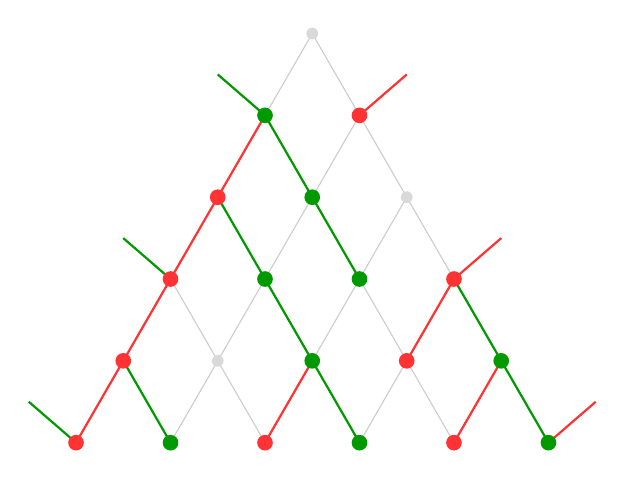
\begin{tikzpicture}[scale=1.2]
  \tikzstyle{reddot}=[circle, fill=red!80, inner sep=2pt]
  \tikzstyle{greendot}=[circle, fill=green!60!black, inner sep=2pt]
  \tikzstyle{emptydot}=[circle, fill=gray!30, inner sep=1.5pt]
  \tikzstyle{redline}=[red!80, thick]
  \tikzstyle{greenline}=[green!60!black, thick]
  \tikzstyle{grayline}=[gray!40, thin]
  \draw[redline] (0.000, 0.000) -- (0.500, 0.866);
  \draw[grayline] (1.000, 0.000) -- (1.500, 0.866);
  \draw[greenline] (1.000, 0.000) -- (0.500, 0.866);
  \draw[redline] (2.000, 0.000) -- (2.500, 0.866);
  \draw[grayline] (2.000, 0.000) -- (1.500, 0.866);
  \draw[grayline] (3.000, 0.000) -- (3.500, 0.866);
  \draw[greenline] (3.000, 0.000) -- (2.500, 0.866);
  \draw[redline] (4.000, 0.000) -- (4.500, 0.866);
  \draw[grayline] (4.000, 0.000) -- (3.500, 0.866);
  \draw[greenline] (5.000, 0.000) -- (4.500, 0.866);
  \draw[redline] (0.500, 0.866) -- (1.000, 1.732);
  \draw[grayline] (1.500, 0.866) -- (2.000, 1.732);
  \draw[grayline] (1.500, 0.866) -- (1.000, 1.732);
  \draw[grayline] (2.500, 0.866) -- (3.000, 1.732);
  \draw[greenline] (2.500, 0.866) -- (2.000, 1.732);
  \draw[redline] (3.500, 0.866) -- (4.000, 1.732);
  \draw[grayline] (3.500, 0.866) -- (3.000, 1.732);
  \draw[greenline] (4.500, 0.866) -- (4.000, 1.732);
  \draw[redline] (1.000, 1.732) -- (1.500, 2.598);
  \draw[grayline] (2.000, 1.732) -- (2.500, 2.598);
  \draw[greenline] (2.000, 1.732) -- (1.500, 2.598);
  \draw[grayline] (3.000, 1.732) -- (3.500, 2.598);
  \draw[greenline] (3.000, 1.732) -- (2.500, 2.598);
  \draw[grayline] (4.000, 1.732) -- (3.500, 2.598);
  \draw[redline] (1.500, 2.598) -- (2.000, 3.464);
  \draw[grayline] (2.500, 2.598) -- (3.000, 3.464);
  \draw[greenline] (2.500, 2.598) -- (2.000, 3.464);
  \draw[grayline] (3.500, 2.598) -- (3.000, 3.464);
  \draw[grayline] (2.000, 3.464) -- (2.500, 4.330);
  \draw[grayline] (3.000, 3.464) -- (2.500, 4.330);
  \draw[greenline] (0.000, 0.000) -- (-0.500, 0.433);
  \draw[redline] (5.000, 0.000) -- (5.500, 0.433);
  \draw[greenline] (1.000, 1.732) -- (0.500, 2.165);
  \draw[redline] (4.000, 1.732) -- (4.500, 2.165);
  \draw[greenline] (2.000, 3.464) -- (1.500, 3.897);
  \draw[redline] (3.000, 3.464) -- (3.500, 3.897);
  \node[reddot] at (0.000, 0.000) {};
  \node[greendot] at (1.000, 0.000) {};
  \node[reddot] at (2.000, 0.000) {};
  \node[greendot] at (3.000, 0.000) {};
  \node[reddot] at (4.000, 0.000) {};
  \node[greendot] at (5.000, 0.000) {};
  \node[reddot] at (0.500, 0.866) {};
  \node[emptydot] at (1.500, 0.866) {};
  \node[greendot] at (2.500, 0.866) {};
  \node[reddot] at (3.500, 0.866) {};
  \node[greendot] at (4.500, 0.866) {};
  \node[reddot] at (1.000, 1.732) {};
  \node[greendot] at (2.000, 1.732) {};
  \node[greendot] at (3.000, 1.732) {};
  \node[reddot] at (4.000, 1.732) {};
  \node[reddot] at (1.500, 2.598) {};
  \node[greendot] at (2.500, 2.598) {};
  \node[emptydot] at (3.500, 2.598) {};
  \node[greendot] at (2.000, 3.464) {};
  \node[reddot] at (3.000, 3.464) {};
  \node[emptydot] at (2.500, 4.330) {};
\end{tikzpicture}

\end{tabular}
\end{document}